\chapter{Materials and experimental apparatus}
\label{ch:materials_apparatus}%
% Aim: 12-15 pages. What was tested and with what. No results here.

This chapter describes the materials tested and the apparatus used to test them. The materials are the lunar highlands simulant LHS-1, granular ice made in the laboratory, and their mixtures. The apparatus is a uniaxial compaction vessel in which a sample, laterally confined by a rigid steel wall, is loaded axially by a piston driven by pressurised oil, at temperatures down to $-40\,^\circ$C. The characterisation of the apparatus (friction, compliance, transducer range and drift) and the test procedure are presented in Chapter~\ref{ch:characterisation}.

% Items marked TODO in the comments must be checked in the laboratory before submission.

% ---------------------------------------------------------------------------
\section{Materials}
\label{sec:materials}
% ---------------------------------------------------------------------------

\subsection{Lunar highlands simulant LHS-1}
\label{subsec:lhs1}

The regolith component of all samples is the lunar highlands simulant LHS-1, produced by Exolith Lab. Its mineralogy, grain size and density, as given by the manufacturer and by independent tests, are summarised in Table~\ref{tab:lhs1} (Section~\ref{sec:regolith}). The properties used in the data reduction of this thesis are:
\begin{itemize}
    \item grain density $\rho_s = 2.75$\,g/cm$^3$, from the manufacturer's specification sheet~\cite{exolithLHS1};
    \item mean and median grain size of 90 and 60\,$\mu$m, with grains from below 1\,$\mu$m up to 1\,mm~\cite{exolithLHS1}.
\end{itemize}
The grain density directly affects the volume of solids and therefore the void ratio. Independent measurements on another batch gave 2.81\,g/cm$^3$~\cite{agarwal2023}; the effect of this uncertainty on the void ratio is discussed in Section~\ref{sec:uncertainty}.
% TODO: batch number and date of the simulant used; if possible, measure rho_s of the batch with a pycnometer.

LHS-1 contains glass and a large fraction of fine particles, and adsorbs water vapour from the air. Since any adsorbed water would freeze and add to the ice content of the samples, the simulant was oven-dried before use and stored in sealed containers.
% TODO: drying temperature and duration (e.g. 105 C for 24 h), container type, storage location.
Before mixing with ice, the dry simulant was cooled in the cold room, so that it would not melt the ice grains on contact.

\subsection{Granular ice}
\label{subsec:ice}

The ice was prepared following the laboratory's standard procedure, which produces ice of controlled grain size and with minimal impurities. It consists of two steps.

\paragraph{Bulk ice.} Deionised water is placed in a metal bucket inside an insulated container with an opening at the bottom, and is frozen slowly at about $-5\,^\circ$C over about 48\,h. Freezing therefore proceeds from the bottom upwards, and dissolved gas and impurities are pushed towards the last liquid at the top. This bubble-rich top part is scraped away, and the clear ice below is stored in the cold room.

\paragraph{Seed ice.} In the cold room (about $-20$ to $-25\,^\circ$C), clear pieces of bulk ice are broken with a saw and a hammer and ground in a food processor for about 5 minutes. The resulting powder is passed through a stack of sieves (2\,mm, 1\,mm, 500\,$\mu$m, 250\,$\mu$m, 160\,$\mu$m), helped by a brush and a plastic scraper. The fraction retained between the 500\,$\mu$m and 250\,$\mu$m sieves is used in this work. Coarser and finer fractions are stored and reused.

The sieved ice grains are angular fragments of polycrystalline or single-crystal ice. Their size range, 250--500\,$\mu$m, is similar to that of the ice used in the firn compaction experiments carried out on the same vessel (210--500\,$\mu$m)~\cite{skarbek2025data}, so that the pure-ice tests of this thesis can be compared directly with those data. The ice is stored in sealed containers in the cold room and used within a few days, to limit sintering and grain growth before testing.
% TODO: confirm storage time between sieving and testing.

The density of ice at the test temperatures is taken as $\rho_i = 0.917$\,g/cm$^3$; its variation between $-10$ and $-40\,^\circ$C is below 0.5\% and is neglected.

\subsection{Ice--regolith mixtures}
\label{subsec:mixtures}

\paragraph{Composition.} The composition of the mixtures is defined by the gravimetric ice content $w_i = m_i/m_s$ (Equation~\eqref{eq:wi}), where $m_i$ and $m_s$ are the masses of ice and dry simulant. Because the ice and the simulant have very different densities, the same composition corresponds to very different fractions by volume. The volume fraction of ice in the solid phases,
\begin{equation}
    \phi_i = 1-\phi_s = \frac{m_i/\rho_i}{m_i/\rho_i + m_s/\rho_s},
    \label{eq:phii}
\end{equation}
is the quantity that controls whether the simulant grains are in contact or dispersed in the ice (Section~\ref{subsec:ice_content_def}). Table~\ref{tab:compositions} gives the correspondence between the different measures for some representative compositions.

\begin{table}[H]
    \centering
    \caption{Correspondence between measures of ice content for mixtures of ice ($\rho_i = 0.917$\,g/cm$^3$) and LHS-1 ($\rho_s = 2.75$\,g/cm$^3$).}
    \label{tab:compositions}
    \begin{tabular}{|c|c|c|c|}
        \hline
        $w_i = m_i/m_s$ & $x_i = m_i/(m_i+m_s)$ & $\phi_i$ (volume of ice / volume of solids) & $\phi_s$ \\
        \hline
        0.10 & 0.091 & 0.23 & 0.77 \\
        0.20 & 0.167 & 0.38 & 0.62 \\
        0.35 & 0.259 & 0.51 & 0.49 \\
        0.50 & 0.333 & 0.60 & 0.40 \\
        1.00 & 0.500 & 0.75 & 0.25 \\
        \hline
    \end{tabular}
\end{table}

A mixture with equal masses of ice and simulant ($w_i = 1$) contains three times more ice than simulant by volume, whereas equal volumes ($\phi_i = 0.5$) correspond to $w_i\approx0.35$. In this thesis the compositions are always reported as $w_i$, with the corresponding $\phi_i$.

\paragraph{Preparation.} The mixtures are prepared in the cold room. For each sample:
\begin{enumerate}
    \item the masses of ice and dry simulant needed for the target composition and initial void ratio are computed from the sample cross-section and the target height (see below), and weighed with a balance of 0.01\,g resolution;
    % TODO: confirm balance resolution.
    \item the two components, both at cold-room temperature, are mixed in a closed container by gentle shaking and stirring with a spatula until the colour is uniform;
    \item the mixture is poured into the sample chamber of the vessel, already cooled to the test temperature, on top of the lower porous frit, in a few layers. Each layer is lightly tamped to reach the target height and to give the sample enough integrity to be handled.
\end{enumerate}
% TODO: check that steps 2-3 describe what was actually done (mixing time, number of layers, tamping tool).

\paragraph{Homogeneity.} The simulant grains (median 60\,$\mu$m) are much finer than the ice grains (250--500\,$\mu$m). When mixed dry, fine particles tend to coat the coarser grains and fill the gaps between them, but they can also segregate when the mixture is poured, the fines moving downwards. Pouring in layers and limiting the free fall of the mixture reduce segregation. The homogeneity of the samples was checked qualitatively after each test, by observing the colour of the sample along its height after extraction.
% TODO: describe the post-test inspection actually done; if possible, cut the sample into slices and weigh/melt them to measure ice content along the height.

\paragraph{Initial state.} The initial void ratio of the sample is computed from its measured height $H_0$ and from the masses of the two components:
\begin{equation}
    e_0 = \frac{H_0}{H_s} - 1, \qquad H_s = \frac{1}{A}\left(\frac{m_i}{\rho_i} + \frac{m_s}{\rho_s}\right),
    \label{eq:e0}
\end{equation}
where $A$ is the cross-sectional area of the sample chamber (Section~\ref{sec:vessel}) and $H_s$ is the height of solids, that is, the height the sample would have with no pores. In Equation~\eqref{eq:e0} both ice and simulant are treated as solids, so $e_0$ is the void ratio of the mixture, with air as the only pore fluid. The initial height is measured once the sample is in the chamber, from the depth of the upper frit below the top of the vessel (Section~\ref{subsec:geometry}). Since the masses are measured before mixing, any loss of material during preparation, or sublimation during the test, is checked by weighing the sample at the end of the test.

% ---------------------------------------------------------------------------
\section{Uniaxial compaction vessel}
\label{sec:vessel}
% ---------------------------------------------------------------------------

\subsection{Overview}

The tests were performed in a uniaxial compaction vessel (Parr Instrument Company, model A1000G) that was modified in the laboratory to operate below freezing~\cite{skarbek2025data}. The vessel and its ancillary systems are shown schematically in Figure~\ref{fig:vessel}. A cylindrical sample sits in a steel sample chamber between two porous frits and rests on a steel spacer. It is loaded from above by a steel piston, whose upper end is in a chamber filled with low-viscosity silicone oil. When oil is pumped into the chamber, the piston is pushed down and compresses the sample. Since the chamber wall is rigid, the sample cannot expand laterally and is compressed under oedometric ($K_0$) conditions.

\begin{figure}[H]
    \centering
    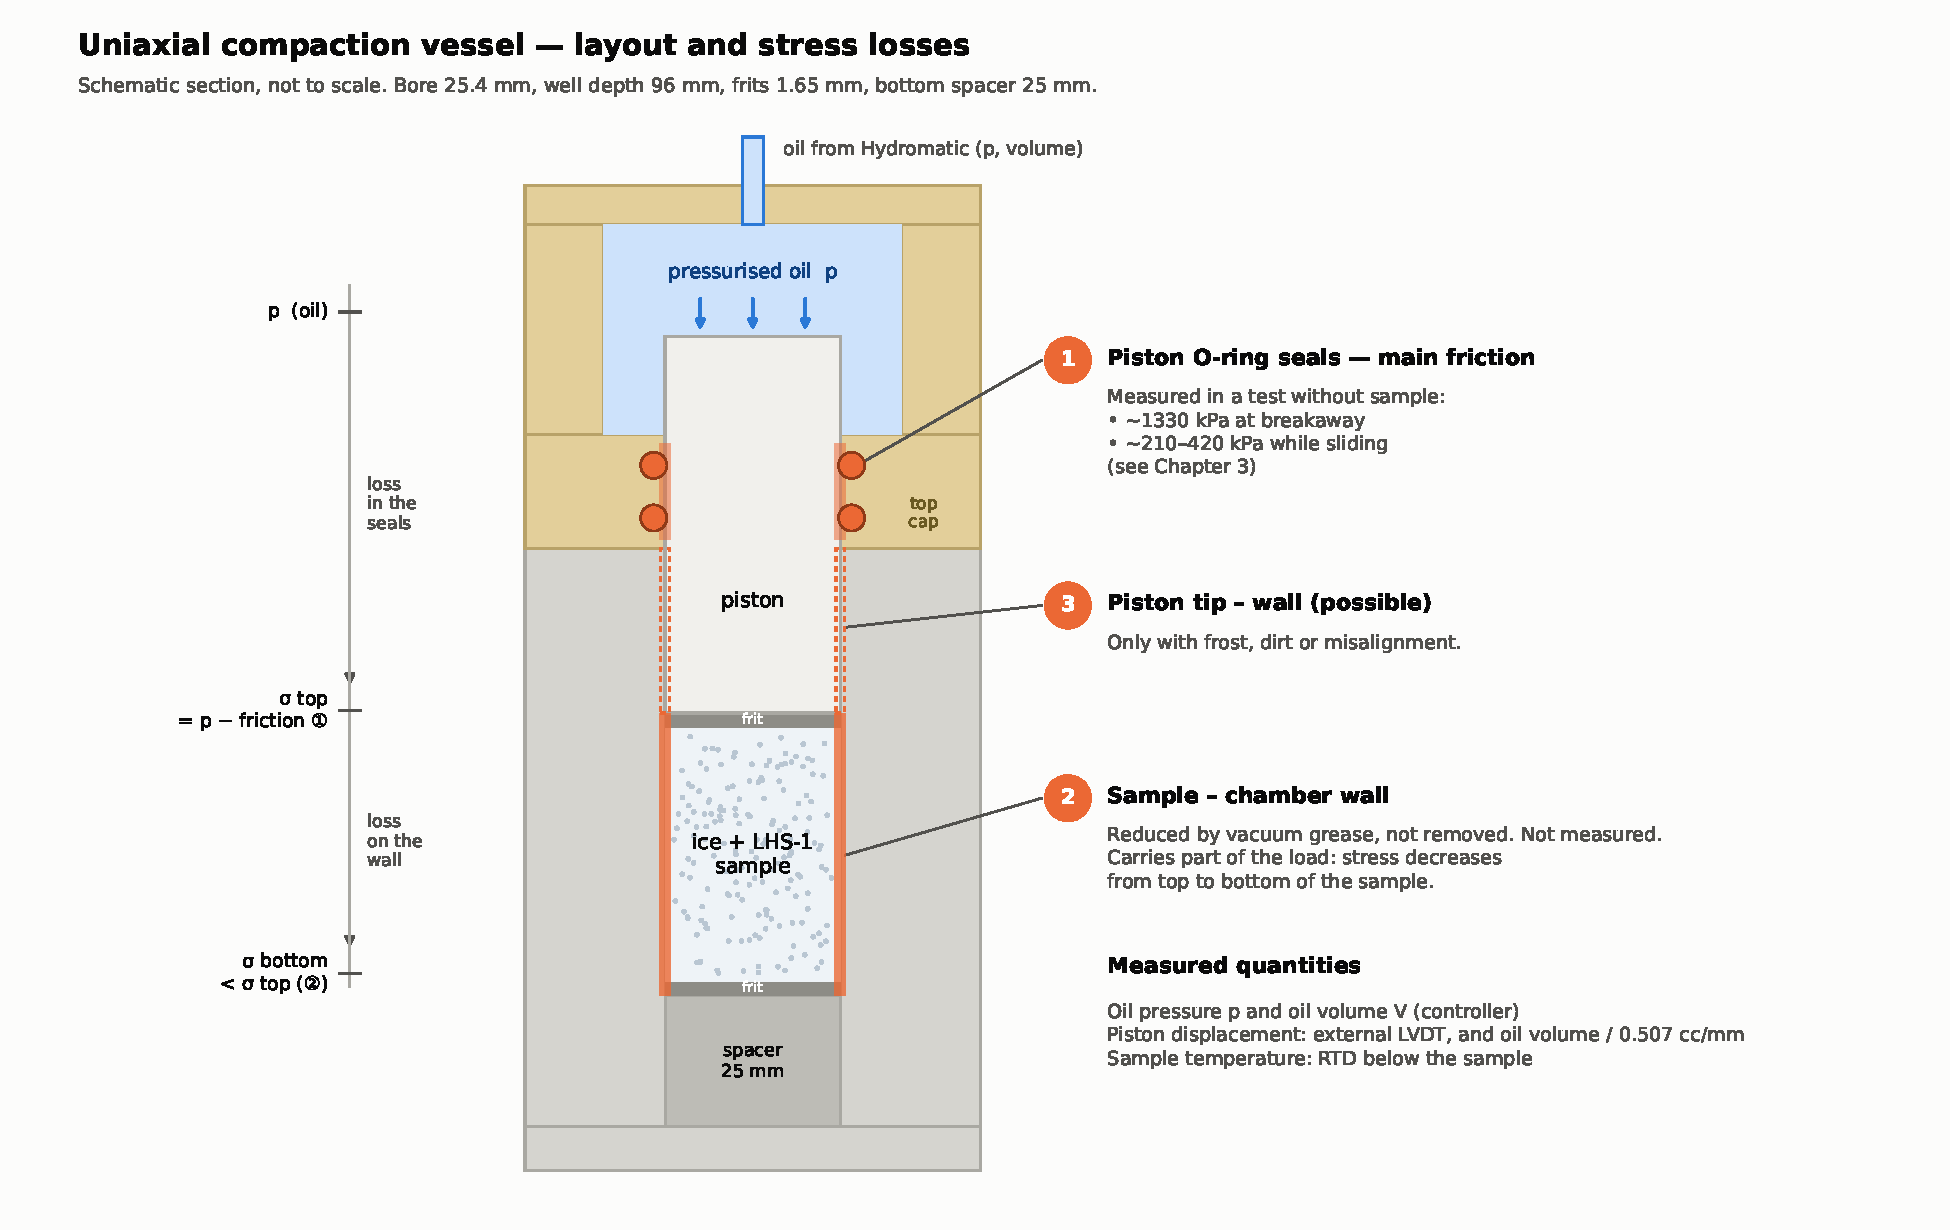
\includegraphics[width=\textwidth]{Images/vessel_schematic.pdf}
    \caption{Schematic cross-section of the uniaxial compaction vessel (not to scale), with the zones where friction reduces the stress transmitted from the oil to the sample. The friction terms are quantified in Chapter~\ref{ch:characterisation}.}
    \label{fig:vessel}
\end{figure}

The vessel can be operated in two ways:
\begin{itemize}
    \item \textbf{pressure control}: the oil pressure is kept constant, so that the axial force on the piston is constant and the sample creeps under a nominally constant stress. This is the mode used in all compaction tests;
    \item \textbf{volume control}: a given volume of oil is pumped into the chamber, which imposes a given piston displacement. This mode was used only to characterise the seal friction (Chapter~\ref{ch:characterisation}).
\end{itemize}

\subsection{Geometry}
\label{subsec:geometry}

\paragraph{Sample chamber.} The sample chamber is a cylindrical bore with a diameter of 25.4\,mm (1\,inch), so that the cross-sectional area of the sample is $A = 5.07$\,cm$^2$. Its depth, measured from the top surface of the vessel to the top of the bottom assembly, is $W = 96$\,mm. The bottom assembly is threaded into the lower end of the vessel and consists of a plug that forms the floor of the chamber, a 25\,mm steel spacer and a threaded closure. It can be removed to extract the sample at the end of the test.
% TODO: confirm the reference surfaces for W = 96 mm with a drawing or a direct measurement.

\paragraph{Porous frits.} The sample is placed between two porous metal frits with a diameter equal to that of the chamber and a thickness $t_f = 1.65$\,mm. The frits distribute the load uniformly over the sample faces and let air escape from the pores during compaction. They are cleaned in an ultrasonic bath, dried and weighed before each test, and cooled in the freezer before being placed in contact with the sample.

\paragraph{Piston.} The piston is a steel cylinder with the same diameter as the chamber, which runs through the top cap of the vessel. It has an axial bore that vents the air expelled from the sample. Its upper end is in the oil chamber and is sealed by O-rings housed in the top cap. Since the oil acts on the full cross-section of the piston, a volume of oil $\Delta V$ pumped into the chamber moves the piston by
\begin{equation}
    \Delta x = \frac{\Delta V}{A} = \frac{\Delta V}{0.507\,\mathrm{cm^3/mm}},
    \label{eq:dx_volume}
\end{equation}
if the oil circuit were perfectly rigid. Equation~\eqref{eq:dx_volume} is the basis of the oil-volume measurement of displacement (Section~\ref{subsec:displacement}); the corrections for the compliance of the circuit are presented in Chapter~\ref{ch:characterisation}.

\paragraph{Sample height.} After the sample is placed in the chamber and the upper frit is placed on it, the depth $d$ from the top surface of the vessel to the top of the upper frit is measured with the depth rod of a caliper. The initial height of the sample is then
\begin{equation}
    H_0 = W - d - 2\,t_f.
    \label{eq:H0}
\end{equation}
At the end of the test, the height of the extracted sample is measured with a caliper, and the length of the piston protruding from the top cap is recorded. The two measurements give independent checks of the final height.

\paragraph{Wall preparation.} Before each test, the chamber, the piston and the threads are cleaned with isopropanol, to remove residual grease and moisture that could freeze on the threads. The chamber wall is then coated with a thin layer of vacuum grease, which reduces the friction between sample and wall and makes extraction easier. Before a new sample is inserted, the piston must be pushed back into its housing, expelling the oil used in the previous test back through the oil line. This is done by striking the piston with a rubber mallet while holding the top cap, with the oil line open.

\subsection{Loading system}
\label{subsec:loading}

\paragraph{Pressure/volume controller.} The oil pressure and volume are controlled by a stand-alone pressure/volume controller (Hydromatic 28-WF45SG, Controls S.p.A.). It consists of a piston pump driven by a stepper motor along a linear track, with a volume capacity of 250\,cm$^3$, and controlled by a touch-screen panel. Its main specifications are~\cite{hydromatic2018}:
\begin{itemize}
    \item maximum pressure 3500\,kPa;
    \item pressure resolution 0.1\,kPa;
    \item volume resolution 0.001\,cm$^3$, equivalent through Equation~\eqref{eq:dx_volume} to a piston displacement of 2\,$\mu$m;
    \item operating temperature of the controller +15 to +40\,$^\circ$C, so that the controller sits in the laboratory, outside the freezer.
\end{itemize}

The controller runs a programmed sequence of up to 15 steps. Each step consists of a ramp to a target value of pressure or volume, with a prescribed duration, followed by a hold at the target for a prescribed time. For each ramp and hold, the user selects whether the change in volume is measured and whether the volume reading is reset to zero at the start of the step. The internal data logging can be linear in time, or follow a power law or a geometric progression, so that more readings are taken at the start of a step. Upper and lower pressure limits can be set; when a limit is exceeded, the controller can sound an alarm, hold or stop the test. The upper limit must be set sufficiently above the target pressure, otherwise the overshoot at the end of a fast ramp stops the test (Chapter~\ref{ch:characterisation}).

\paragraph{Oil circuit.} The controller is connected to the vessel by a line that runs from the laboratory into the freezer. The circuit has two valves:
\begin{itemize}
    \item a valve at the wall, which connects the line to the oil reservoir. It is opened when the piston is pushed back between tests, so that the expelled oil can return to the reservoir, and closed during tests;
    \item an L-shaped valve inside the freezer, between the line and the vessel. When it is closed, the controller can pressurise the line up to the vessel without loading the sample; opening it applies the pressure to the piston.
\end{itemize}
The second valve allows the sample to be loaded with a step of stress: the line is first brought to the target pressure with the valve closed, and the valve is then opened. This is the loading procedure used in the firn compaction experiments and adopted in this thesis (Chapter~\ref{ch:characterisation}).

\paragraph{Range of axial stress.} The maximum oil pressure of 3.5\,MPa is also, to a first approximation, the maximum axial stress on the sample, since the oil acts on a piston of the same diameter as the sample. The stress actually transmitted to the sample is lower, because part of the force is taken by the friction of the piston seals and by the friction between sample and wall (Figure~\ref{fig:vessel}). In this thesis the target pressures range from 0.5 to 3.4\,MPa.

\subsection{Displacement measurement}
\label{subsec:displacement}

\paragraph{LVDT.} The displacement of the piston is measured outside the vessel by a linear variable differential transformer (LVDT), mounted on the top cap and touching a flat plate fixed to the piston. The LVDT has a resolution of about 1\,$\mu$m~\cite{skarbek2025data}. Its calibration is valid only for negative readings, that is, with the core pushed in beyond its zero position: the LVDT must be set at the start of each test so that the reading is negative, and the readings close to zero are unreliable. In the configuration used, the reading saturates at about $-19.6$\,mm.
% TODO: LVDT model, nominal stroke and calibration factor.
The usable stroke of the LVDT is therefore smaller than the total compaction of a loose sample, which can exceed 20\,mm. How the LVDT is set to cover the time-dependent stage of the test is described in Chapter~\ref{ch:characterisation}.

\paragraph{Oil volume.} The volume of oil delivered by the controller provides a second, independent measurement of the piston displacement through Equation~\eqref{eq:dx_volume}. It covers the whole stroke of the piston, including the fast compaction at the start of the test, which the LVDT cannot follow when it goes out of range. The oil volume is affected by the compressibility of the oil, the expansion of the line under pressure, possible leaks and temperature changes of the oil in the line. These effects are measured and corrected as described in Chapter~\ref{ch:characterisation}.

\subsection{Temperature control}
\label{subsec:temperature}

The sample chamber is surrounded by an outer jacket through which chilled methanol is circulated by a refrigerated circulator (Julabo Magio MS-1000F). The temperature is measured by a resistance temperature detector (RTD) placed close to the bottom surface of the sample, which is also the control sensor of the circulator. The whole vessel is housed in a chest freezer, which provides additional insulation and reduces the temperature gradient along the vessel. With this setup the sample temperature can be controlled down to $-40\,^\circ$C with a precision of 0.05\,$^\circ$C~\cite{skarbek2025data}.

Before loading, the sample is left in the closed vessel for at least one hour to reach a uniform temperature. Only the vessel is temperature-controlled: the controller and most of the oil line are at laboratory temperature, which changes between day and night. The effect of these changes on the oil volume is discussed in Chapter~\ref{ch:characterisation}.

\subsection{Data acquisition}
\label{subsec:daq}

The data are recorded by a data logger (Geodatalog 8, Controls S.p.A.) controlled by the DATACOMM~2 software on a laboratory computer, through a dedicated Ethernet connection~\cite{geodatalog2020}. The logger has eight independent input channels with an effective resolution of 131\,000 points and can sample up to 500 readings per second per channel. Three quantities are recorded:
\begin{itemize}
    \item the LVDT displacement, from an analogue input channel of the logger;
    \item the oil pressure and the oil volume, read from the pressure/volume controller through the network, so that all three are recorded with the same time base.
\end{itemize}
All tests were logged at 1\,Hz, the same rate as the firn compaction experiments. This rate resolves the fast compaction in the first seconds after loading and gives files of manageable size (about 225\,000 rows for a test of 62\,h). The controller also stores its own record of pressure and volume, which is used as a backup.
% TODO: check that the computer is not connected to the external network during tests (lab rule), and mention it if relevant.

The sample temperature is recorded by the circulator.
% TODO: check whether the RTD temperature is logged with the other channels or only displayed by the circulator; if logged, give the channel and rate.
